\documentclass[10pt]{article}
\usepackage[polish]{babel}
\usepackage[utf8]{inputenc}
\usepackage[T1]{fontenc}
\usepackage{amsmath}
\usepackage{amsfonts}
\usepackage{amssymb}
\usepackage[version=4]{mhchem}
\usepackage{stmaryrd}
\usepackage{graphicx}
\usepackage[export]{adjustbox}
\graphicspath{ {./images/} }

\title{KLASY PIERWSZE I DRUGIE }

\author{}
\date{}


\begin{document}
\maketitle
\begin{enumerate}
  \item Rozwiąż w liczbach całkowitych równanie
\end{enumerate}

\[
x(x+1)+(x+1)(x+2)+\cdots+(x+9)(x+10)=2022 x+2023
\]

\begin{enumerate}
  \setcounter{enumi}{1}
  \item Początkowo na tablicy napisane są liczby 2 oraz 5. Ruch polega na zastąpieniu jednej z dwóch liczb napisanych na tablicy ich sumą. Czy po wykonaniu pewnej liczby ruchów można uzyskać sytuację, w której na tablicy napisane są dwie kolejne liczby naturalne? Odpowiedź uzasadnij.
  \item Czy długości boków, na które dzielą się dwie przecinające się cięciwy okręgu mogą wyrażać się czterema kolejnymi liczbami naturalnymi?\\
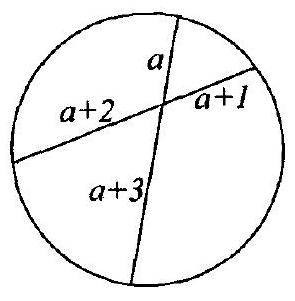
\includegraphics[max width=\textwidth, center]{2024_11_21_b929c47ff1092b2cac26g-1}
\end{enumerate}

\section*{KLASY TRZECIE I CZWARTE}
\begin{enumerate}
  \item Dana jest liczba całkowita \(n>1\). Udowodnij, że liczba
\end{enumerate}

\[
n^{4}+4^{n}
\]

jest złożona.\\
2. Udowodnij, że jeśli liczby całkowite \(a, b, c\) spełniają równanie

\[
(a+3)^{2}+(b+4)^{2}-(c+5)^{2}=a^{2}+b^{2}-c^{2}
\]

to wspólna wartość obu stron jest kwadratem liczby całkowitej.\\
3. Udowodnij, że istnieje nieskończenie wiele parami różnych liczb całkowitych \(a, b, c\) i \(d\), że liczby

\[
a^{2}+2 c d+b^{2} \text { oraz } c^{2}+2 a b+d^{2}
\]

są kwadratami.


\end{document}